\documentclass[a4paper, 12pt]{article}
% Allow the usage of graphics (.png, .jpg)
\usepackage[pdftex]{graphicx}
\graphicspath{ {./images/} }
\usepackage{apacite}
\usepackage[T1]{fontenc}
\usepackage{url}
\usepackage{amsmath}
\usepackage{algorithm}
\usepackage{algpseudocode}
\usepackage{subcaption}

\makeatletter
\def\BState{\State\hskip-\ALG@thistlm}
\renewcommand{\ALG@name}{Compute Distance}
\renewcommand{\thealgorithm}{}
\makeatother

% set line spacing
\usepackage{setspace}
\setlength{\parindent}{0pt}
\setlength{\parskip}{2ex}
\linespread{1.3}

% caption
\usepackage{caption} 
\captionsetup[table]{skip=10pt}

\usepackage{tocloft} % for list of equations
% define list of equations
\newcommand{\listequationsname}{\Large{List of Equations}}
\newlistof{myequations}{equ}{\listequationsname}
\newcommand{\myequations}[1]{
   \addcontentsline{equ}{myequations}{\protect\numberline{\theequation}#1}
}
\setlength{\cftmyequationsnumwidth}{2.3em}
\setlength{\cftmyequationsindent}{1.5em}

% Comment the following line to NOT allow the usage of umlauts
\usepackage[utf8]{inputenc}
%custom margins
\usepackage[]{vmargin}
\setpapersize{A4}	
\setmarginsrb{35mm}{30mm}{30mm}{20mm}{0pt}{0mm}{12pt}{13mm}
% Correct hyphenation in urls
\usepackage{url}
% Support long tables
\usepackage[]{longtable}
\usepackage{ltablex}
\usepackage{adjustbox}
%Pretty bibliography in UEF format
\usepackage{natbib}
% verbatim code listings
\usepackage{listings}
%Unobtrusive in document links
\usepackage{hyperref}
\hypersetup{
    colorlinks,
    citecolor=black,
    filecolor=black,
    linkcolor=black,
    urlcolor=black
}
%%%%%%%%%%%%%%%%%%%%%%%%%%UEF FORMAT%%%%%%%%%%%%%%%%%%%%%%%%%%%%%%%%%


\begin{document}

% do cover pages
%Fill these in and they'll propagate across the title page. Remember to keep the space at the end!
\def \ajankohta {Tammikuu 2014 }
\def \ajankohtaenglish {August 2021 }
\def \authorname {Nguyen To }
\def \thesistitle {Sign Language Recognition }
\def \thesissubtext {Inflated 3D ConvNet  }
\def \campus {Joensuu }
\def \facultyschooleng {School of Computer Science }
\def \facultyschoolfin { }
%FT = PhD, FM = MSc
\def \supervisorsfin { }
\def \supervisorseng {Profressor Xiao-Zhi Gao }

\def \documenttypeeng {Master's Thesis }
\def \documenttypefin { }
%\def \documenttypeeng {Bachelor's Thesis}
%\def \thesistypefin {Kandidaatintutkielma}

%Number of non-cover pages, to last page of references
\def \mypagecount {42 }
\def \myappendixcount {1 }
\def \myappendixpagecount {32 }

\graphicspath{ {./images/} }
%%%%%%%%%%%%%%%%%% TITLE PAGE %%%%%%%%%%%%%%%%%%

\vspace*{3cm}
\vspace{0.5cm}

\begin{center}
\begin{LARGE}\thesistitle \end{LARGE}

\begin{Large}\thesissubtext \end{Large} 

\vspace{1.5cm}

\begin{Large}\authorname \end{Large}

\vspace{\stretch{1}}

{\large
\documenttypeeng
~\\
% to have it in black and white, swap the commented line
\includegraphics[width=7cm]{{UEF logo.png}}\\
% \includegraphics[width=7cm]{UEF_fin_pysty_1_black}\\
Faculty of Science and Forestry\\
\facultyschooleng \\
}
\end{center}

\vspace{0.5cm}

\thispagestyle{empty}

\begin{spacing}{1.0}
\newpage

%%%%%%%%%%%%%%%%%% Abstract page in English %%%%%%%%%%%%%%%%%%

UNIVERSITY OF EASTERN FINLAND, Faculty of Science and Forestry, \campus School of Computing\\
\facultyschooleng \\ \\
Student, \authorname : \thesistitle \\
\documenttypeeng , \mypagecount p.\\
Supervisors of the \documenttypeeng : \supervisorseng \\
\ajankohtaenglish \\


Abstract:

Effective communication is considered as the foremost fundamental of human skills. However, more than 5\% of the world's population is suffering from disabling hearing loss, as indicated by the World Health Organization (WHO). There is hence a communication gap between the hearing-impaired community, whose primary means of communication is sign language, and others who are not privy with this language. To this end, Sign Language Recognition could be an essential instrument which utilizing vision-based technology and helps the hearing-impaired communicate with the society with ease, thereby diminishing the verbal exchange barrier. The first step in interpreting and analyzing communication via gestures is word-level sign language recognition (WSLR). Recognizing signs from recordings maybe a tough challenge due to the fact that the meaning of a word is determined by a combination of subtle body movements, hand gestures, and other actions. Be that as it may, with the significant advancement of technology, notably Convolutional Neural Network (CNN), in this paper, an Inflated 3D Networks (I3D), a 3D video categorization solution are used to method as an answer of WSLR.


% Key words English

% Edellisellä sivulla olevien suomenkielisten avainsanojen käännökset

~\\ % Tämä tekee tyhjän rivin; älä editoi tätä pois
Keywords:
Sign Language, Continuous Sign Language, Sign Language Recognition, Classification,
Vidieo Classification, Recognition

% CR-luokat

% ACM-luokitus löytyy Computing Reviews -lehden jokaisen
% vuosikerran ensimmäisestä numerosta sekä verkosta
% osoitteesta http://www.acm.org/class/

% Ota omat luokkasi tuoreimmasta vuosikerrasta.

CR Categories (ACM Computing Classification System,
1998 version): A.m, K.3.2\\

\end{spacing}

\newpage


%%%%%%%%%%%%%%%%%% Foreword/Preface %%%%%%%%%%%%%%%%%%

\section*{Preface}
The basis for the project initially originated from my ardor for developing better methods of sign language recognition. The hearing-impaired community's life has changed considerably over the past half-century as a result of policy adjustments and latest technological tendencies, yet the road to find a viable answer for word-level sign language recognition (WSLR) keeps on being a drawn out circumstance. It is my passion to not solely find out, however to develop tools to bridge the communication gap between the deaf community and the society. This project follows the reference and citation guidelines of the "Quo Valdis, Action Recognition? A New Model and the Kinetics Datasets” by a group of Jo\~{a}o Carreira and Andrew Zisserman.

In truth, I could not have achieved my current level of success without a strong support group. To begin with, I wish to express my sincere thanks to my supervisor, Profressor Xiao-Zhi Gao, for his excellent guidance, valuable input and support throughout the entire period.
Furthermore, I would also like to thank Li Dongxu for his enormously valued assistance in collecting data for this study.
Especially with respect Cong Phan, a Phd candidate at Griffith University who gave a great help by offering several useful insights and recommendations. 
And finally, I am grateful to Mai Khanh Nguyen Ngoc. She stood by my side and provided me with the support I needed to complete this thesis. 
\newpage

%%%%%%%%%%%%%%%%%% Abbrieviations %%%%%%%%%%%%%%%%%%

\section*{List of Abbreviations}

\begin{tabular}{lp{12.5cm}}

ACM & Association for Computing Machinery \\

ISY & Itä-Suomen yliopisto \\

UEF & University of Eastern Finland\\

WSLR & Word-level Sign Language Recognition\\

I3D & Two -Stream Inflated 3D Convolutional Network\\

CNN & Convolutional Neural Network\\

LSTM & Long-short Term Memory\\

TGCN & Temporal Graph Convolutional Network\\

\end{tabular}

\newpage


% ----------------- Table of Contents -------------

% Älä tee seuraavaan mitään muutoksia:

\setlength{\parskip}{0ex}

\tableofcontents
\newpage

\listoftables
\newpage

\listoffigures
\newpage

\setlength{\parskip}{2ex}

\pagenumbering{gobble} % arabic(1234) numbering, autoreset to 1


\section{Introduction}
Sign Language, any methods of communicating by bodily motions, particularly with hands and arms, that is utilized when verbal communication is either difficult or undesirable. Sign language can consist of a series of overly-exaggerated facial expressions, shrugs, or hand gestures; or it can be a fine and delicate mix of hand signals that are complemented by facial expressions and words spelt out using a manual alphabet. When a deaf person or someone speaking a different language is communicating with someone who is hearing, using sign language can help connect the parties. \citep{signlanguagedefinition2020}. The public has neither the time nor the patience to learn sign language, which is complicated and time-consuming to learn and practice. Additionally, there are also many language and culture-specific \citep{holtz2014reading} (e.g Germany, Japanese) constraints which will hinder the widespread adoption of sign language.
Significant advances in deep learning (DL) and improvements in device capabilities, such as computation power, memory capacity, power usage, sensor resolution, and optics, have improved the performance and cost-effectiveness of vision-based applications, allowing them to spread more quickly in the market place.
For this reason, it is interesting to examine sign language recognition (SLR), which automatically translates sign language and aids deaf-mute individuals in communicating with others in their life

Back to the history of 90s, Yann LeCun et al. published "Gradient-Based Learning Applied to Document Recognition", which is widely considered to be the most popular AI article from the era. This paper was the first modern application of convolutional neural networks to be developed.
Since then, more and more sophisticated models trained on ever-larger datasets have been built using the convenient approach of convolutional neural networks. Especially in the field of Computer Vision - Human-based activity recognition, there are many methods can be applied to solve the problem, from traditional convolutional neural networks such as CNN-RNN, CNN-LSTM to RestNetCRNN, Conv3D and state-of-the-art networks e.g Pose-TGCN, I3D.
Inheriting the idea of using two-stream I3D network, which is based 2D ConvNet \citep{carreira2017quo}, presented by Carreira and Zisserman, this project is re-implement the model with a slightly modification inside. It might not be better when comparing with other models, however during the project, I have got many experience and broaden my knowledge on the field of Deep Learning. 

\subsection{Problem}
As same as other human-based activity recognition, SRL also shares some common problems such as background clutter, lightning or lightning changing in a video, motion blur, angle of camera, changing scale. 
SRL, on the other hand, is a more difficult task than ordinary action recognition. Firstly, sign language relies on a combination of global body movement and subtle hand/arm gesture. Additionally, depending on how many times they are repeated, same gestures might have different meanings. SRL might be more difficult to examine because of different states of motions and signers such as localism, gesture speed, preferred hand or physical form. Finally, it is also expensive to collect additional data from many signers even though it is desirable \citep{jiang2021skeleton}.

As described above, the datasets that uses for training SLR are limited, even the number of samples inside each dataset. The table below describes some datasets that normally use for researching.

\begin{table}[ht!]
    \centering
    \def\arraystretch{1}%
    \caption{Sign Language Datasets.}
    \resizebox{\textwidth}{!}{
        \begin{tabular}{|l|l|l|l|l|l|}
            \hline \textbf{Dataset} & \textbf{Language} & \textbf{Classes} & \textbf{Samples} & \textbf{Data Type} & \textbf{Language Level} \\
            \hline CSL Dataset I & Chinese & 500 & 125,000 & Video \& Depth from Kinect & Isolated \\
            \hline CSL Dataset II & Chinese & 100 & 25,000 & Videos \& Depth from Kinect & Continuous \\
            \hline RWTH-PHOENIX-Weather 2014 & German & 1,081 & 6,841 & Videos & Continuous \\
            \hline RWTH-PHOENIX-Weather 2014 T & German & 1,066 & 8,257 & Videos & Continuous \\
            \hline ASLLVD & American & 3,300 & 9,800 & Videos(multiple angles) & Isolated \\
            \hline ASLLVD-Skeleton & American & 3,300 & 9,800 & Skeleton & Isolated \\
            \hline SIGNUM & German & 450 & 33,210 & Videos & Continuous \\
            \hline DGS Kinect 40 & German & 40 & 3,000 & Videos(multiple angles) & Isolated \\
            \hline DEVISIGN-G & Chinese & 36 & 432 & Videos & Isolated \\
            \hline DEVISIGN-D & Chinese & 500 & 6,000 & Videos & Isolated \\
            \hline DEVISIGN-L & Chinese & 2000 & 24,000 & Videos & Isolated \\
            \hline LSA64 & Argentinian & 64 & 3,200 & Videos & Isolated \\
            \hline GSL isol. & Greek & 310 & 40,785 & Videos \& Depth from RealSense & Isolated \\
            \hline GSL SD & Greek & 310 & 10,290 & Videos \& Depth from RealSense & Continuous \\
            \hline GSL SI & Greek & 310 & 10,290 & Videos \& Depth from RealSense & Continuous \\
            \hline IIITA -ROBITA & Indian & 23 & 605 & Videos & Isolated \\
            \hline PSL Kinect & Polish & 30 & 300 & Videos \& Depth from Kinect & Isolated \\
            \hline PSL ToF & Polish & 84 & 1,680 & Videos \& Depth from ToF camera & Isolated \\
            \hline BUHMAP-DB & Turkish & 8 & 440 & Videos & Isolated \\
            \hline LSE-Sign & Spanish & 2,400 & 2,400 & Videos & Isolated \\
            \hline Purdue RVL-SLLL & American & 39 & 546 & Videos & Isolated \\
            \hline RWTH-BOSTON-50 & American & 50 & 483 & Videos(multiple angles) & Isolated \\
            \hline RWTH-BOSTON-104 & American & 104 & 201 & Videos(multiple angles) & Continuous \\
            \hline RWTH-BOSTON-400 & American & 400 & 843 & Videos & Continuous \\
            \hline WLASL & American & 2,000 & 21,083 & Videos & Isolated \\
            \hline
        \end{tabular}
    }
    \label{table:1}
\end{table}

Time segmentation is another issue for SLR as it is difficult to distinguish different kinds of sign language while signers make gestures continuously to describe a phrase or a sentence \citep{xiao2020multi}.
Word-level sign recognition, an integral part of comprehending sign language phrases and sentences, is also extremely difficult task itself:
\begin{itemize}
    \item The meaning of signals is primarily determined by the mix of bhand actions, body motions and head positions, and small variations in these elements can result in a variety of interpretations.
    \item With the same gesture, depend on the natural languages and context, they might have different meaning. It is also possible for nouns and verbs from the same lemma to share the same sign. These nuances are not effectively reflected by the small-scale datasets that are currently available (Figure 1) \citep{li2020word}.
    \item The number of signs that are used on daily basis is enormous, it could be thousands. In comparison, tasks such as gesture and action recognition have just had a few hundred categories. The scalability of recognition algorithms is significantly hampered as a result.
\end{itemize}

\begin{figure}[hbt!]
    \centering
    \begin{subfigure}[b]{0.3\textwidth}
        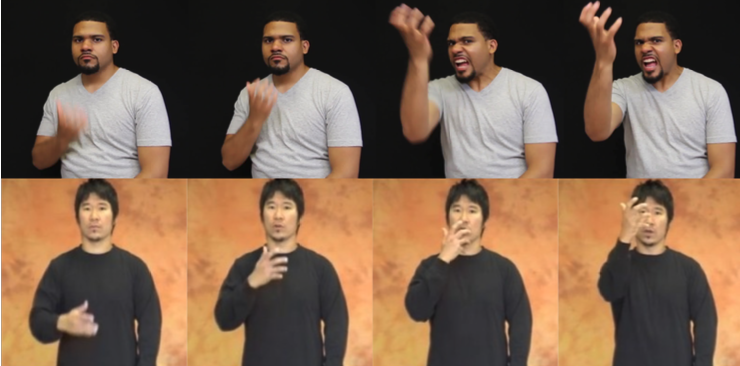
\includegraphics[width=\textwidth]{fig2a.png}
        \caption{\textbf{"Scream"} is performed slightly different by different signers}
        \label{Figure 1.a}
    \end{subfigure}
    \hfill
    \begin{subfigure}[b]{0.3\textwidth}
        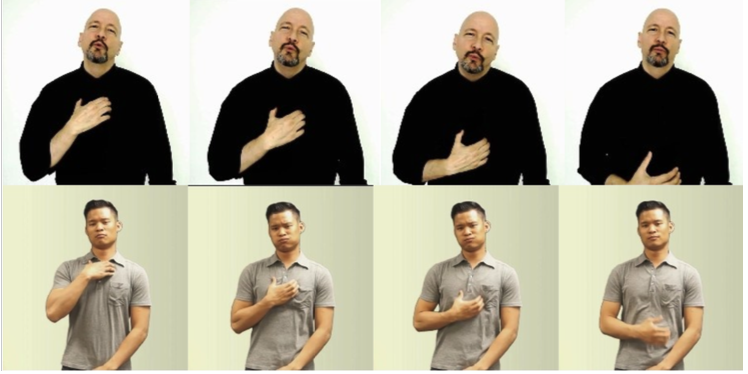
\includegraphics[width=\textwidth]{fig2b.png}
        \caption{The verb \textbf{"Wish"} (top) and the adjective \textbf{"Hungry"} (bottom) have same gesture}
        \label{Figure 1.b}
    \end{subfigure}
    \hfill
    \begin{subfigure}[b]{0.3\textwidth}
        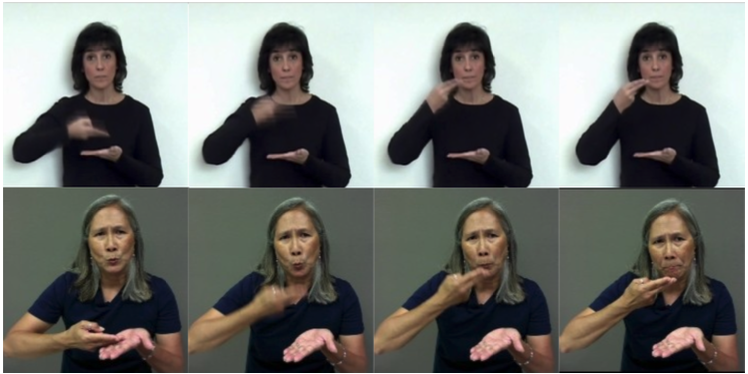
\includegraphics[width=\textwidth]{fig2c.png}
        \caption{\textbf{"Rice"} (top) and \textbf{"Soup"} (bottom) have same gesture}
        \label{Figure 1.c}
    \end{subfigure}
    \caption{Common occurrence of ambiguity and variation signing}
    \label{Figure 1}
\end{figure}

\subsection{Thesis scope and target}
In fact, the researching of SLR, including isolated (word-level) and continuous (phrase or sentences), has yielded significant results and developed rapidly in recent years \Citep{lim2019isolated,li2018deep,mercanoglu2021chalearn}.
So this project aims to understand the architecture of I3D model, focuses on the methodology of training, evaluating the network with given dataset. A further objective of the project is getting familiar with libraries and frameworks of Deep Learning which is built for Python environment, and also other related topics such as image processing, data labelling, development tools e.g Google Colab, Anaconda, Jupyter Notebook.
Regarding data and dataset, the project gave a comprehensive overview of organizing data, loading, splitting data for training and testing purpose.

Finally, in terms of the topic's aim, this thesis primarily focuses on enhancing the accuracy of the dataset with the two-stream I3D network. Because of the limitation of facilities, such as hardware, and time-consuming of training process, the project only used the WLASL dataset. 
In order to reduce the consumption of training time, as well as to test the effectiveness of I3D network, the dataset is divided into many sub-datasets which have 100 classes, 300 classes, 1000 classes and 2000 classes.

\section{Model}
\subsection{Methodology of video classification and CNNs}
A video is a collection of multi images which are represented by sequential. Therefore, the main idea of clarifying an action or object inside a video is analyzing frame by frame. In details, the general procedure of video recognition \citep{sivic2003video,niebles2010modeling} contains three key stages. 
The video is first divided into regions \citep{liu2009recognizing} based on the places that are easy to characterize in visual terms. This is done by either sampling regions densely \citep{wang2013action} or, if there are few areas of interest \citep{laptev2005space}, by using a sparse sampling technique. 
In the next step, the characteristics are merged into a video level description with defined size. One common method is to train a K-means dictionary and then evaluate all the features. This allows to gather visual words during the duration of the video and then arrange them into histograms of various spatio-temporal positions and extents \citep{karpathy2014large,laptev2008learning}.
Finally, a classifier (such as an SVM) is trained to discriminate between the classes of interest with the resulting "bag of words.".

CNN, a single neural network which emulates the process of human brain \citep{lecun1998gradient} offer an approach that combines 3 phases into an end-to-end training from the raw value of pixels to the output classifiers. By using restricted connection across layers (local filters), parameter sharing (convolutions), and specific local invariance-building neurons (max pooling), the spatial structure of pictures is specifically exploited. Recently with the outstanding of GPU, CNNs can now scale the networks with millions variables, resulting in significant developments in object recognition \citep{girshick2014rich}, image classification \citep{krizhevsky2017imagenet}, scene annotation. The use of CNNs has piqued the interest of many in the computer vision research community \citep{zha2015exploiting}, and it has been demonstrated that CNN-based methods can reach state-of-the-art performance on various of complex image datasets \citep{sharif2014cnn}.

\begin{figure}[hbt!]
    \centering
    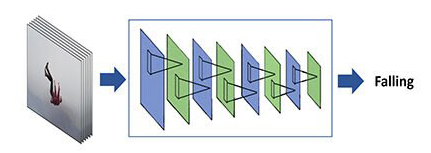
\includegraphics[width=1\textwidth]{Video_classification_and_human_activity_recognition.jpg}
    \caption{An example of video classification}
    \label{Figure 2}
\end{figure}

\subsection{Some models to solve video recognition problems}
\subsubsection{ConvNet-LSTM}
LSTM network and CNNs have been researched widely but independently previously. While CNNs are able to give spatially specific information, LSTM networks are good at producing temporally comprehensive results \citep{mutegeki2020cnn}. As a result, the use of CNN-LSTM networks is extensively employed for time series data, and is particularly useful for video datasets that have a time dimension.

\begin{figure}[hbt!]
    \centering
    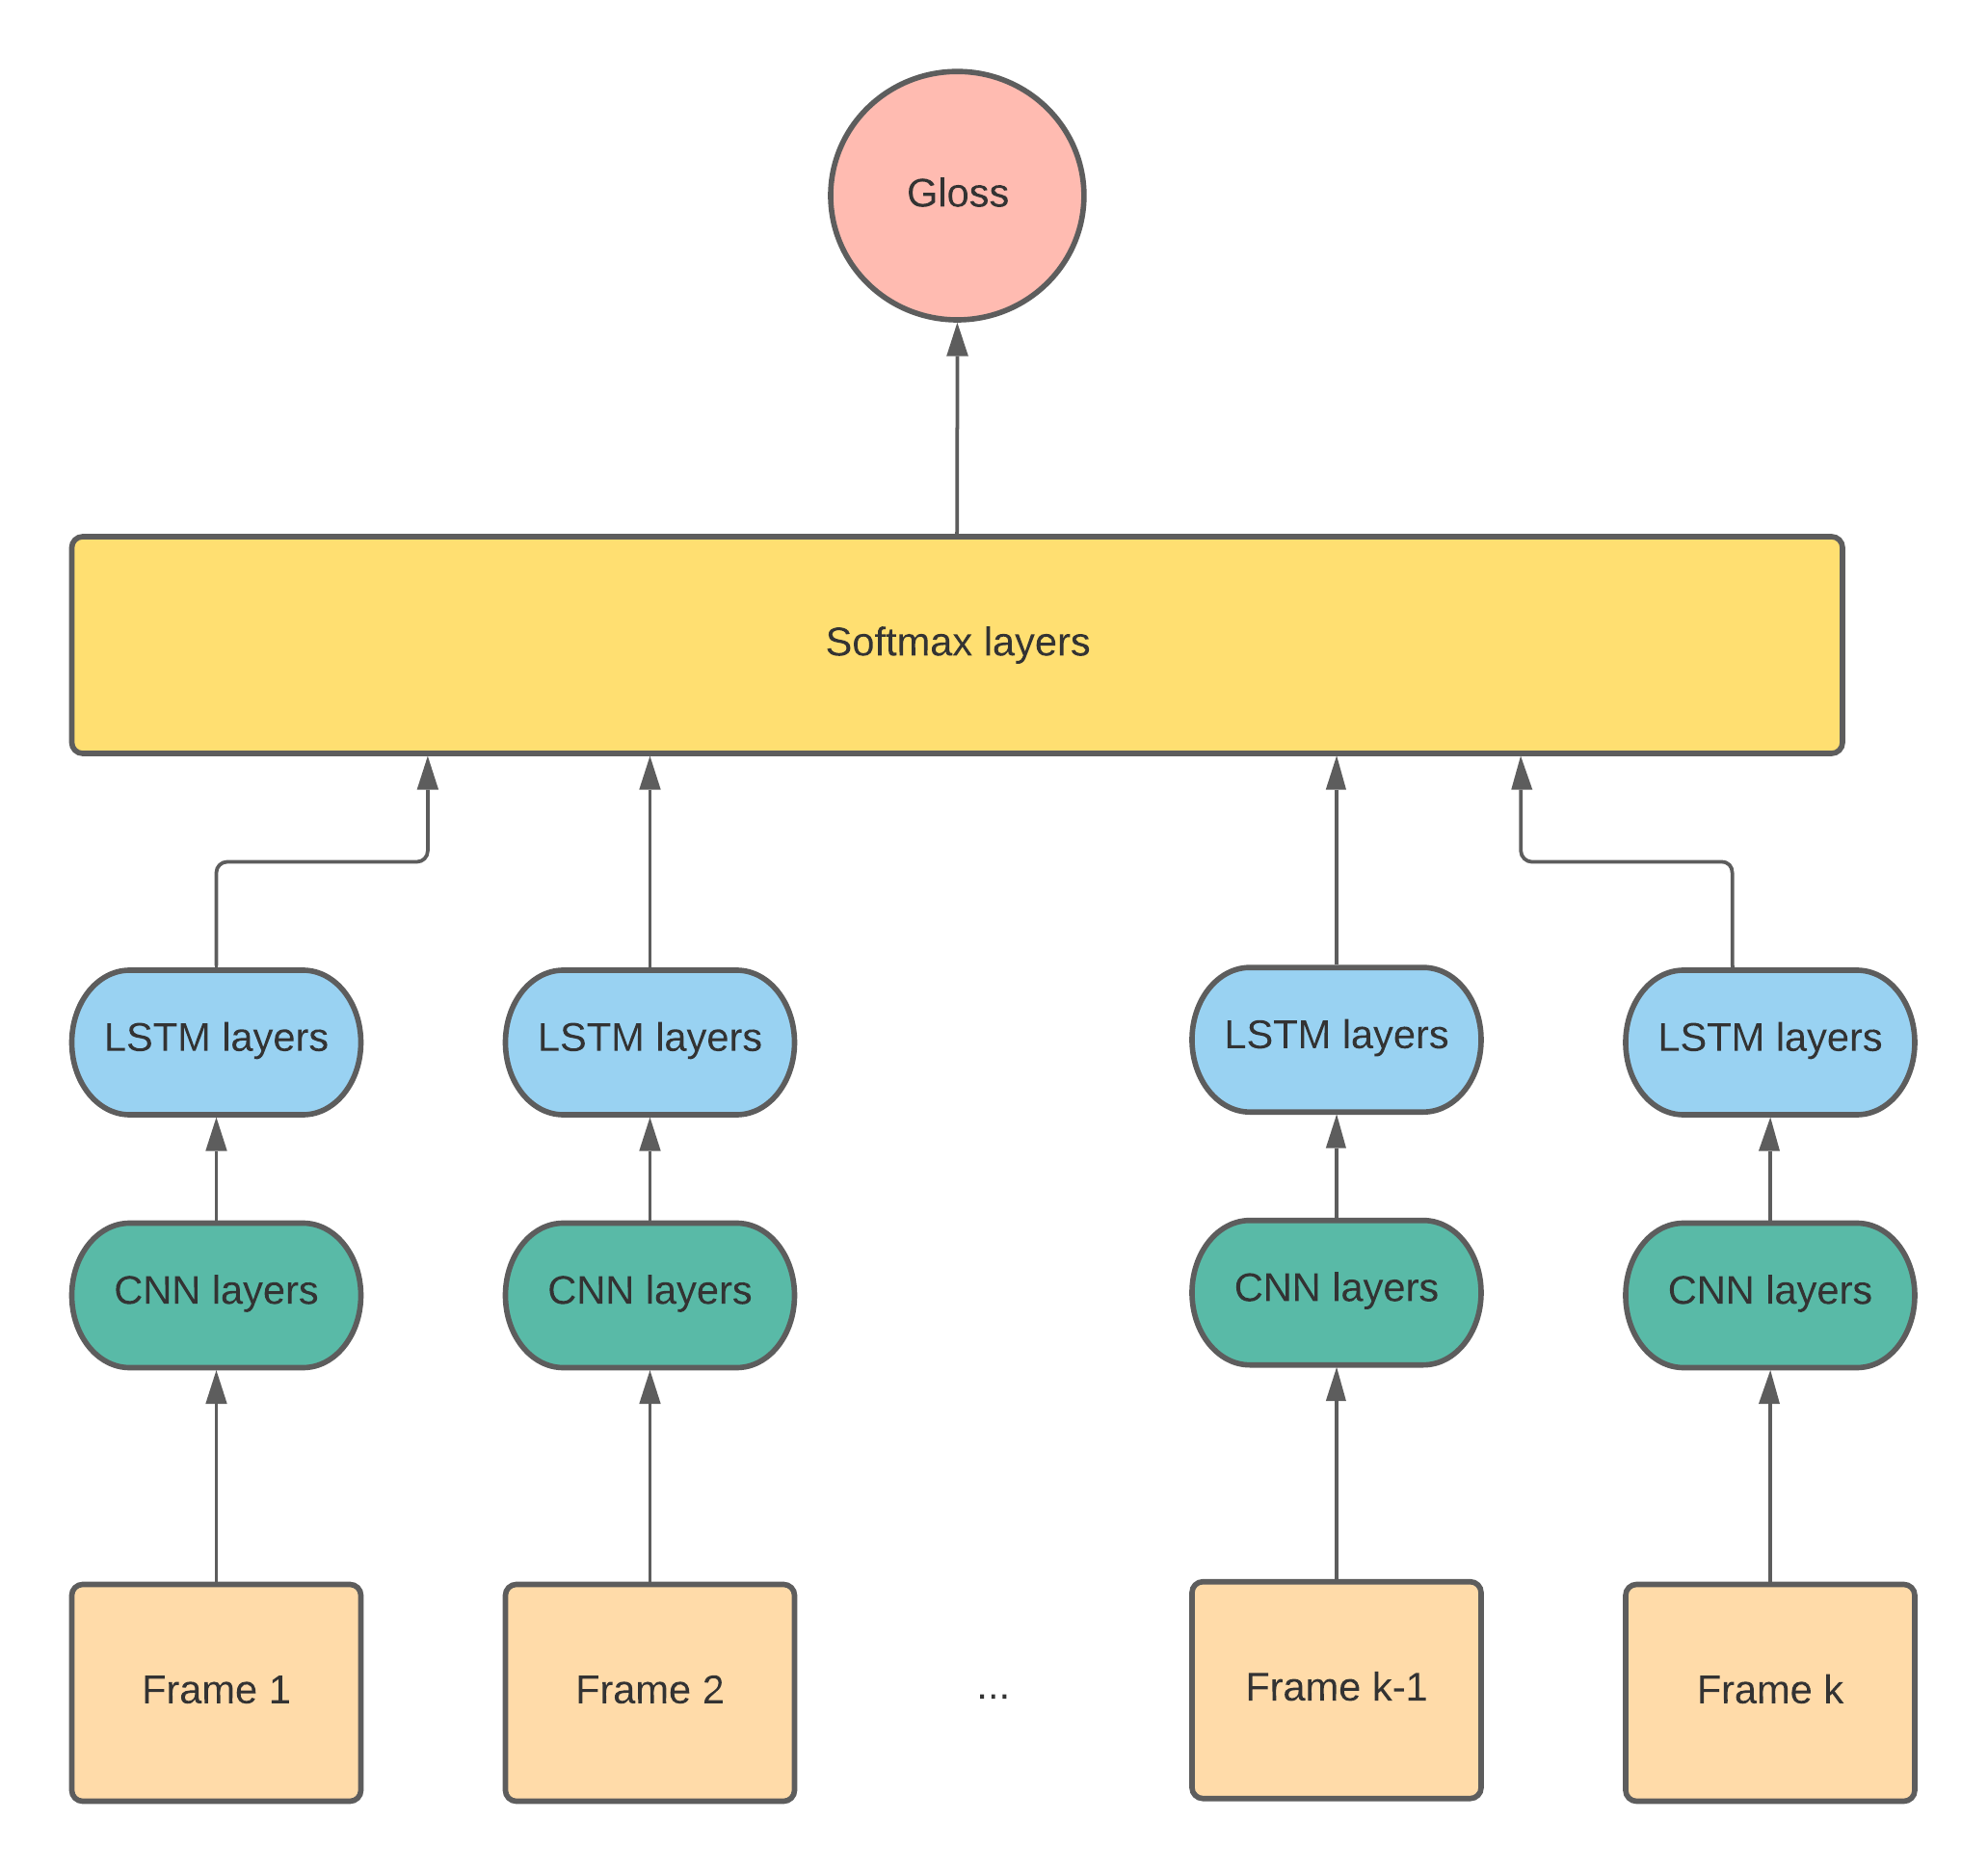
\includegraphics[width=0.75\textwidth]{CNN-LSTM.png}
    \caption{CNN-LSTM model}
    \label{Figure 3}
\end{figure}

In the model of ConvNet-LSTM, features are extracted separately from each frame of a video through a CNN network \citep{karpathy2014large}. Then they are feeded into a LSTM layer \citep{yue2015beyond,donahue2015long}, which is capable of providing stage encoding and temporal ordering. Finally, a fully connected layer is put on the top for classifer.

\subsubsection{3D ConvNet}
Extended from 2D ConvNet, in which convolutions exclusively generate features based on spatial dimensions, 3D ConvNet computes features in the spatial as well as temporal dimensions. Convolution using a 3D kernel is done by convolving a cube of several frames to get a 3D result. This architecture has the additional advantage of making the feature maps in the convolution layer linked to several contiguous frames in the preceding layer, which aids in the capture of motion information \citep{Ji20133DCN}. The use of 3dConvNet have been exploited in many researchs \citep{tran2015learning,taylor2010convolutional}. 

With \textit{\begin{math} c \times l \times h \times w \end{math}} size of a video (c is a number of channel, l is a number of frames, h and w are corresponding to height and width of each frame),
kernel size for 3D convolution and pooling are denoted by the notation \textit{\begin{math}d \times k \times k\end{math}}, where \textit{d} is the kernel temporal depth and \textit{k} is kernel spatial size, 3D ConvNet networks are programmed to accept video clips as inputs and predict the class label that correlate to \textit{n} classes based on datasets \citep{tran2015learning}.

\begin{figure}[hbt!]
    \centering
    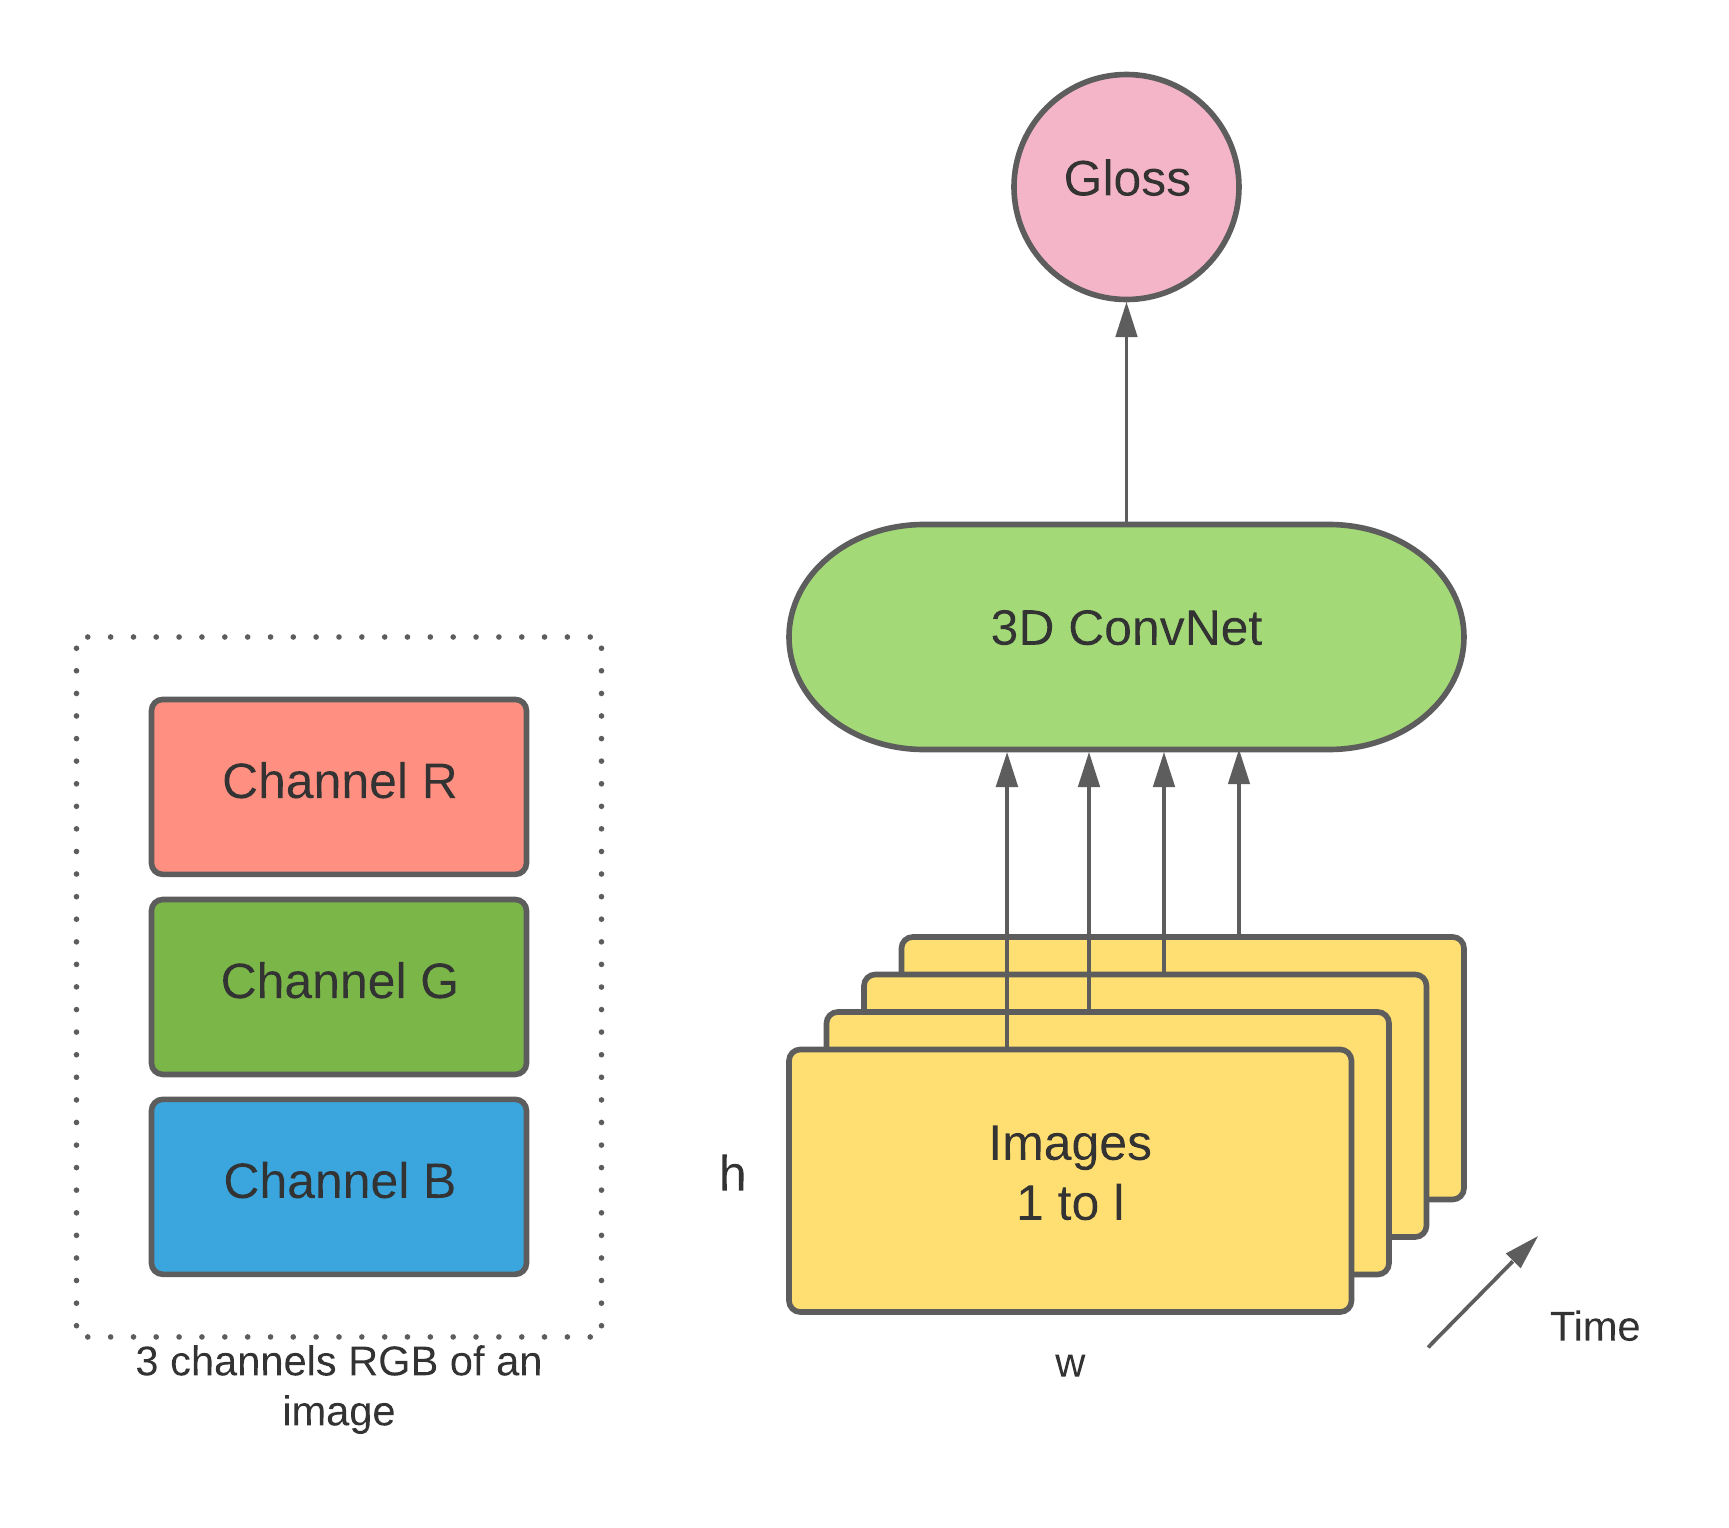
\includegraphics[width=0.75\textwidth]{3D ConvNet Model.png}
    \caption{An example of 3D ConvNet with RGB video as input}
    \label{Figure 4}
\end{figure}

\subsubsection{Two-stream network}
Introduced by Simonyan and Zisserman et al, a model which uses an individual RGB frame and an external n-frame optical flow, was shown extremely high performance on benchmarks, while also being efficient to train and test \citep{simonyan2014two}. In details, a video data is separeted into two streams, spatial stream and temporal stream. The spatial stream can spot motion in static frames, whereas the temporal stream is trained to perceive motion in images as optical flows, both of them are developed with ConvNet \citep{simonyan2014two}.

\begin{figure}[hbt!]
    \centering
    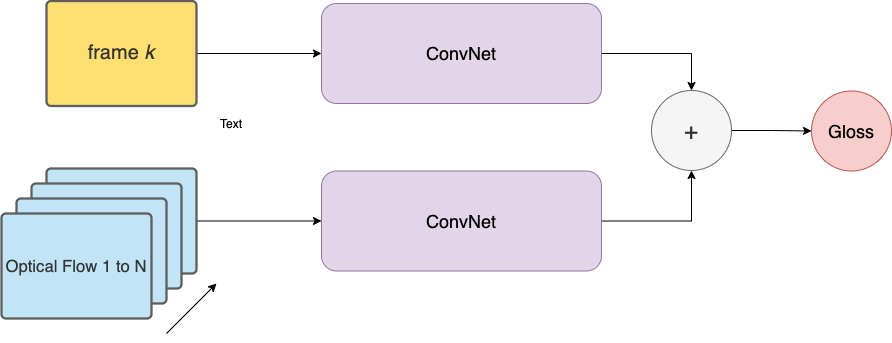
\includegraphics[width=0.75\textwidth]{Two-stream ConvNet Model.png}
    \caption{Two-stream 3D ConvNet model}
    \label{Figure 5}
\end{figure}

The result shown by Simonyan and Zisserman indicates that using optical flow for training a temporal dimension is outperform than training on static frames \citep{karpathy2014large}.

An extended version of two-stream network, 3D-Fused Two-Stream, is using a 3D ConvNet which can learn patterns related to temporal directly \citep{carreira2017quo}. The model of 3d-Fused Two-Stream is as Figure 6.

\begin{figure}[hbt!]
    \centering
    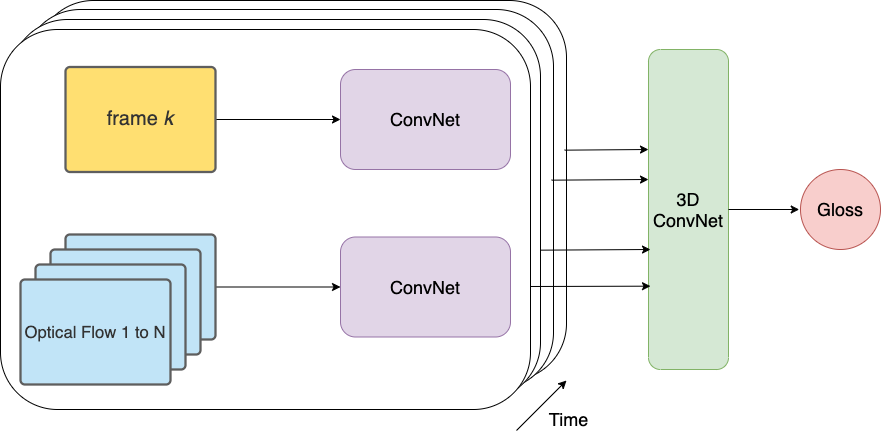
\includegraphics[width=0.75\textwidth]{3D-Fused Two-stream.png}
    \caption{3D-Fused Two-Stream}
    \label{Figure 6}
\end{figure}

\subsection{Model in this study}
With the extendable 2D ConvNet to 3D ConvNet where time dimensions can be added to perform the result, a coming up model is that use two streams of raw images and also optical flow frames. Thus, the temporal patterns is not only studied during the optical flow but also with RGB inputs. As a result, the performance is improved significantly compared with using only RGB stream \citep{carreira2017quo}.

In the method that Zisserman and Carreira proposed, 2 streams are trained independently but the prediction of them are computed as average of 2-stream predictions in test phase. In constrast, in this study, RGB stream and Optical Flow Stream are trained as the same time, and the outputs of them are combined and fed into simple classifier model

\begin{figure}[hbt!]
    \centering
    \begin{subfigure}{0.4\textwidth}
        \centering
        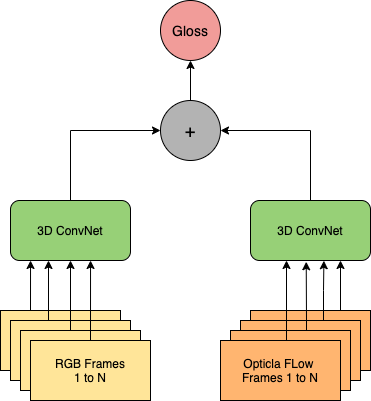
\includegraphics[width=0.6\textwidth]{2-stream I3D Model.png}
        \caption{2-stream 3D ConvNet by Zisserman and Carreira \citep{carreira2017quo}}
        \label{Figure 7.a}
    \end{subfigure}
    \hfill
    \begin{subfigure}{0.4\textwidth}
        \centering
        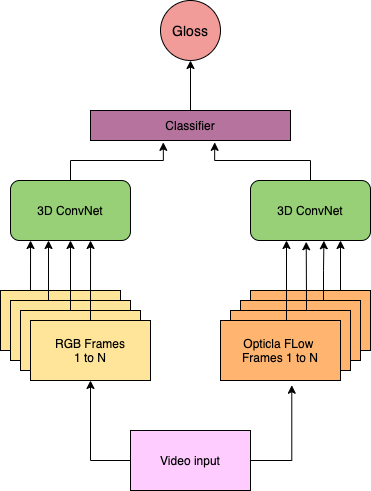
\includegraphics[width=0.6\textwidth]{Modified 2-stream I3D Model.png}
        \caption{Modified 2-stream I3D in this thesis}
        \label{Figure 7.b}
    \end{subfigure}
    \caption{2 models of I3D}
    \label{Figure 7}
\end{figure}

The outputs of an I3D is a list of probability for each frame corresponded to each gloss 

\section{Convolution Neural Network in image classification}
\subsection{Introduction of CNNs}
\subsection{Basic of CNN layers}
\subsection{Kernel vs Filter}
\subsection{1D, 2D, 3D Convolutions}

\section{Techniques for Inflated 3D ConvNet}
\subsection{Inflating 2D ConvNets into 3D ConvNets}
\subsection{2D filters to 3D filters}
\subsection{Space, time and network depth}

\section{Optical flow}
\subsection{Introduction}
Optical flow is a representation of the mobility of a scene environment in relation to an observer's position. In the problem of recognizing human gesture, a static scence in a single frame can lead to an ambiguity in interpreting gesture class.  The movement of human bodies must be taken advantage of in order to have a thorough grasp of the gesture class. There are a variety methods for calculation optical flow from frame to frame, including region-based, energy-based, differential-based, phase-based \citep{marco2018computer}. The differential technique is the most frequently used method, and it is based on the premise of picture brightness constancy \citep{horn1981determining}.

\begin{figure}[hbt!]
    \centering
    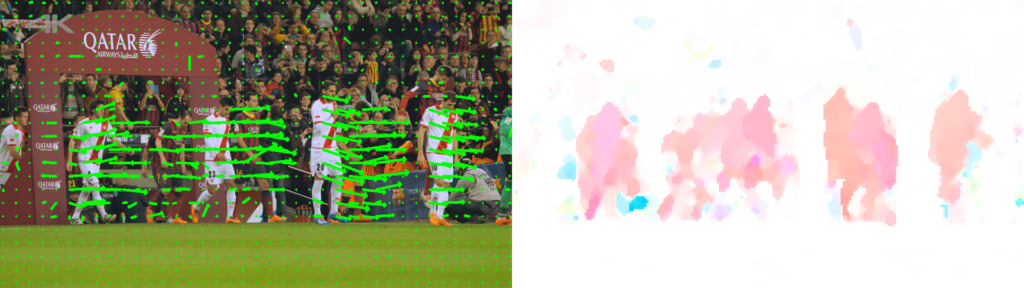
\includegraphics[width=\textwidth]{Football-1024x288.png}
    \caption{Example of an optical flow frame \citep{opticalflowExample}}
    \label{Figure x}
\end{figure}

Assume that the constant brightness of a pixel \textit{(x, y)} in an object does not change; it is not true in reality, however it is reasonable and natural when the time is small enough. Therefore, the image intensity of two continuous frames can expressed by the equation below \citep{o2005optical}.

\begin{equation} \label{eq1}
    I(x, y, t) = I(x +\delta x, y + \delta y, t + \delta t)
\end{equation}
\myequations{Constant intensity assumption}

Then, using Tayloy Series Approximation of the RHS:

\begin{equation} \label{eq2}
    I(x, y, t) = I(x, y, t) + \frac{\partial I}{\partial x}\delta x + \frac{\partial I}{\partial y}\delta y + \frac{\partial I}{\partial t}\delta t
\end{equation}



\subsection{Sparse and Dense Optical Flow}
\subsection{Algorithm for converting RGB video into Optical Flow video}
\subsubsection{Shi-Tomasi Corner Detector and Lucas-Kanade: Sparse Optical Flow}
\subsubsection{Farneback: Dense Optical Flow}
\subsection{Optical Flow in Deep Learning}

\section{Experiment}
\subsection{Datasets}
\subsubsection{Argentina Sign Language Dataset}
\subsubsection{Word Level American Sign Language Dataset}
\subsection{Setup environment}
\subsubsection{Python}
\subsubsection{Goolge Colaboratory}
\subsubsection{Project structure}
\subsection{Results}

\section{Conclusion}


\newpage

% Two common styles, pick one or find alternate bst.
% \citet{john} is like John (1985); \citep{jane} is like (Jane 1985)
%\bibliographystyle{IEEEtranN} % Like this (Jane 1995)
%\bibliographystyle{plain} % Like this [6] 
\newpage
\bibliographystyle{apacite}
\bibliography{document}

\end{document}
